\makeatletter
\def\input@path{{../../}}
\makeatother
\documentclass[../../main.tex]{subfiles}

\graphicspath{
	{../../img/}
	{../img/}
	{img/}
}


\begin{document}
Так как $A, B, C$~--- непрерывные функции (убедиться самостоятельно), то, 
выбрав у $\vec{N} = \pm\left[ \vec r\,'_u, \vec r\,'_v \right]$ конкретный 
знак, в каждой точке поверхности будет определен конкретный вектор нормали. В 
таком случае говорят, что задано \emph{поле нормалей}. В связи с этим, 
поверхности бывают односторонние и двусторонние.

Примерами двусторонних поверхностей являются сфера, эллиптический параболоид и 
т.~д. Примером односторонней поверхности является \emph{лист Мёбиуса} :

\begin{center}
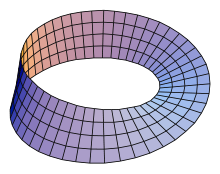
\includegraphics[scale = 0.5]{lec22_0.png}
\end{center}

\[\vec{r}(u, v) = ((2 + u\cos v)\cos2v, \ (2 + u\cos v)\sin2v, \ u\sin v)\]

Рассмотрим лист Мебиуса в точке
\[\vec{r}(0, \ v) = (2\cos v, 2\sin2v, 0) = \vec{r}(0, v + \pi).\]
Получаем
\[\vec{N}(u, v) = (-4\sin v\cos2v, \ -4\sin v\sin2v, \ 4\cos v).\] 

\begin{exc}
 Вычислить $A$, $B$, $C$ самостоятельно.
\end{exc}

\bigskip

Оказывается, что
$\vec{N}(0, v) = -\vec{N}(0, v + \pi).$

\section{Первая квадратичная форма поверхности}

Первая квадратичная форма поверхности играет важную роль для исследования 
поверхностей.

Рассмотрим гладкую двустороннюю поверхность \[\vec{r} = \vec{r}(u,  v) = 
(x(u,  v), \ y(u,  v), z(u,  v)).\]

 \emph{Первой квадратичной формой поверхности} называют величину 
 \begin{gather*}
 I = (d\vec{r})^2 = \left<d\vec{r}, \ d\vec{r}
 \right> = \left<\vec r\,'_udu + \vec r\,'_vdv, \ 
 \vec r\,'_udu + \vec r\,'_vdv\right> = \left<\vec 
 r\,'_u, \ \vec r\,'_u\right>du^2 + 
 2\left<\vec r\,'_u, \ \vec r\,'_v\right>dudv + \\ 
 + \left<\vec r\,'_v, \ \vec r\,'_v\right>dv^2 = 
 Edu^2 + 2Fdudv + Gdv^2,
 \end{gather*}
 где $E$, $G$, $F$~--- \emph{коэффициенты квадратичной формы}
\begin{gather*}
E = \left<\vec r\,'_u, \vec r\,'_u\right> = (x'_u)^2 + (y'_u)^2 + (z'_u)^2, \\
F = \left<\vec r\,'_u, \vec r\,'_v\right> = x'_ux'_v + y'_uy'_v + z'_uz'_v, \\
G = \left<\vec r\,'_v, \vec r\,'_v\right> = (x'_v)^2 + (y'_v)^2 + (z'_v)^2.
\end{gather*}
Введена в употребление Гауссом в середине XIX века.

\section{Вычисление длины кривой на поверхности}

Пусть в области $D$, в которой задана поверхность 
$(u, v) \in D \subset \R^2$, задана кривая 
\[\lambda : \begin{cases}
             u = u(t),\\
             v = v(t),\\
             \alpha \leq t \leq \beta.
            \end{cases}\]
Тогда $\vec{r}(u(t), v(t)) = \vec{\rho}(t) = (x(u(t), v(t)), y(u(t), 
v(t)), z(u(t), v(t)))$ задаёт некоторую кривую на поверхности, когда $t$ 
пробегает отрезок $\left[\alpha, \beta\right]$.

Вычислим длину кривой : 
\[
l = \int\limits_\alpha^\beta\sqrt{(x'_t)^2 + (y'_t)^2 + (z'_t)^2}\,dt = 
\int\limits_\alpha^\beta\sqrt{(dx)^2 + (dy)^2 + (dz)^2} = 
\int\limits_\alpha^\beta  |d\rho| =  \int\limits_\alpha^\beta|d\vec{r}| = 
\int\limits_\alpha^\beta\sqrt{(d\vec{r})^2} = \] 
\[ 
= \int\limits_\alpha^\beta\sqrt{Edu^2 + 2Fdudv + Gdv^2} \text{, где } u = 
u(t), v = v(t). 
\]

\begin{exmp}
На сфере радиуса $r = a$
\[\begin{cases}
 x = a\cos u\cos v,\\
 y = a\cos u\sin v,\\
 z = a\sin u;
 \end{cases}
 -\frac{\pi}{2} \leq u \leq \frac{\pi}{2},\ 
 0\leq v \leq 2\pi\]
задана кривая
\[\begin{cases}
u = t,\\
v = \ln\tg(\frac{\pi}{4} + \frac{t}{2});
\end{cases} \ 0 \leq t \leq 1.\]
Найдём коэффициенты первой квадратичной формы. Для 
сферы $\vec{r} = (x(u, v), y(u, v), z(u, v))$ получаем
\[
\begin{cases}
\vec r\,'_u = (-a\sin u\cos v, -a\sin u\sin v, a\cos v),\\
\vec r\,'_v = (-a\cos u\sin v, a\cos u\cos v, 0).
\end{cases}
\]
Поэтому
\[
E = a^2, \ F = 0, \ G = a^2\cos^2u.
\]
Тогда длина кривой равна
\begin{gather*}
l = \int\limits_0^1\sqrt{a^2d(u(t)^2) + 
a^2\cos^2u(t)d(v(t)^2)} =
\\ =
\int\limits_0^1\sqrt{a^2dt^2 + a^2\cos^2t\left(\frac{1}{2\tg(\frac{\pi}{4} + 
\frac{t}{2})\cos^2(\frac{\pi}{4} + \frac{t}{2})}\right)^2dt^2} = \\
= \left[ 2\tg\left(\frac{\pi}{4} + 
\frac{t}{2}\right)\cos^2\left(\frac{\pi}{4} + \frac{t}{2}\right) = 
2\sin\left(\frac{\pi}{4} + 
\frac{t}{2}\right)\cos\left(\frac{\pi}{4} + \frac{t}{2}\right) = 
\sin\left(\frac\pi2 + t\right) = -\cos(t)
\right] =\\
\int\limits_0^1\sqrt{a^2dt^2 + a^2\frac{\cos^2t}{\cos^2t}dt^2} = 
\int\limits_0^1\sqrt{a^2dt^2 + a^2dt^2} = a\sqrt2.
\end{gather*}
\end{exmp}
\section{Площадь поверхности}
Пусть задана гладкая двусторонняя поверхность $\pi : \vec{r} = \vec{r}(u, v)$, 
 $(u, v) \in D \subset \R^2$:

\begin{center}
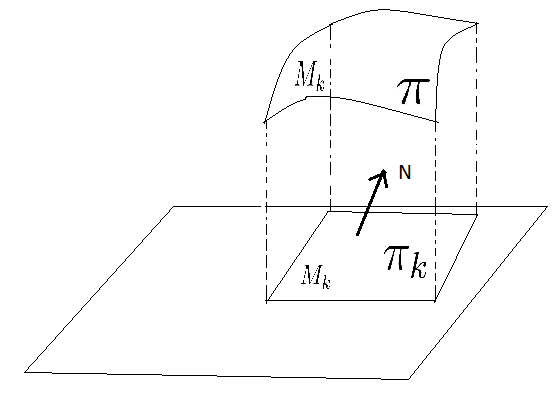
\includegraphics[scale = 1]{lec22_1.png}
\end{center}

Разобьём $\pi$ на части $\pi_k$. На каждом кусочке $\pi_k$
выберем точку $M_k$, и в этой точке построим касательную 
плоскость. Спроецируем $\pi_k$ на касательную плоскость, построенную в точке 
$M_k$. Получим некоторое 
множество $P_k$ с площадью $\Delta S_k$. Тогда \[\text{площадь  } \pi = S_\pi 
\approx \sum\limits_{k=1}^n\Delta S_k,\] то есть \[S_\pi = 
\lim\limits_{\delta\rightarrow0}\sum\limits_{k = 1}^n\Delta S_k,\]
где $\delta$~--- диаметр разбиения. 

\subsection{Вычисление площади}

Если поверхность гладкая и двусторонняя, то она имеет площадь, то есть 
квадрируема. В таких случаях не важно, каким будет разбиение на части $\pi_k$. 
Мы рассмотрим разбиение, построенное с помощью координатных прямых. Рассмотрим 
элемент площади, который соответствует координатным кривым
$\vec{r} = \vec{r}(u, v)$, $\vec{r} = 
\vec{r}(u + \Delta u, v)$, $\vec{r} = \vec{r}(u, v + \Delta v)$. Получаем 
криволинейный четырехугольник:

\begin{center}
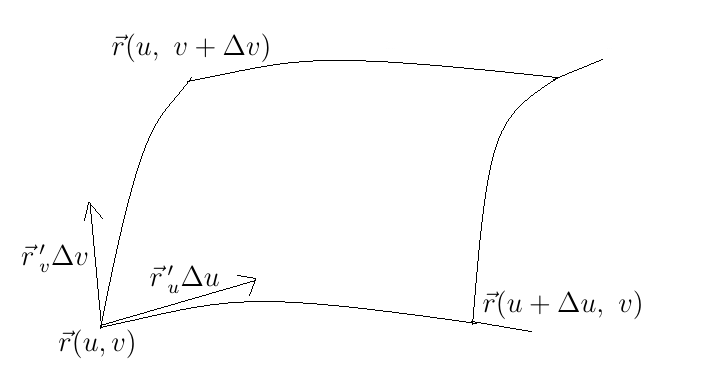
\includegraphics[scale = 1]{lec22_2.png}
\end{center}

Для достаточно мелкого разбиения площадь поверхности приближённо равна площади 
этого элемента. Тогда $\Delta S_k \approx \left|\left[\vec r\,'_u\Delta u, \ 
\vec r\,'_v\Delta v\right]\right| = \left|\left[r'_u, \ 
r'_v\right]\right|\Delta u\Delta v$. 
Суммируя площади и переходя к пределу, получаем
\[S_\pi = \iint\limits_D\left|\left[\vec r\,'_u, \ \vec 
r\,'_v\right]\right|\,du\,dv = \iint\limits_D|\vec{N}|\,du\,dv = 
\iint\limits_D\sqrt{A^2+B^2+C^2}\,du\,dv.\]

Рассмотрим выражение
\begin{gather*}
\left|\left[\vec r\,'_u, \vec r\,'_v\right]\right| = 
\left|\vec r\,'_u\right|\cdot\left|\vec r\,'_v\right| 
\cdot \sin(\vec r\,'_u \ \hat{\ }\  \vec r\,'_v) \implies
\left[\vec r\,'_u, \vec r\,'_v\right]^2 =
(\vec r\,'_u)^2(\vec r\,'_v)^2\sin^2\phi = \\ = EG(1 
- \cos^2\phi) = EG - (|\vec r\,'_u||\vec r\,'_v|\cos\phi)^2 = EG-F^2,
\end{gather*}
т.~е. $|\vec{N}| = \sqrt{EG - F^2}$. Получаем формулу для вычисления площади:
\[
S_\pi = \iint\limits_D\sqrt{EG - F^2}\,du\,dv.
\]

\begin{exmp}
На сфере радиуса $a$, которая задается
\[
\begin{cases}
 x = a\cos u\cos v, \\
 y = a\cos u\sin v,\\
 z = \sin u;
\end{cases}\]
вычислим площадь кусочка, который соответствует
\begin{gather*}
0 \leq u \leq 1, \\ 0 \leq v \leq 1.
\end{gather*}
\[
 S_\pi = \int\limits_0^1du\int\limits_0^1\sqrt{EG-F^2}\,dv = 
 \int\limits_0^1du\int\limits_0^1\sqrt{a^4\cos^2u}\,dv = 
 a^2\int\limits_0^1du\int\limits_0^1\cos u\,dv = a^2\sin u\big|_0^1 = a^2\sin 
 1.
\]
\end{exmp}

\section{Поверхностный интеграл первого рода (ПовИ-1)}

Пусть дана двусторонняя гладкая поверхность $\pi$, и $S$~--- её площадь. \[\pi 
: 
\vec{r} = (x, y, z).\]
Пусть на поверхности задана функция $f(x, y, z)$. 
Рассмотрим разбиение поверхности $\pi$ на кусочки $\pi_k,\ k = \overline{1, 
n}$, $\Delta 
S_k = S_{\pi_k}$, $\delta$~--- диаметр разбиения. На каждом кусочке $\pi_k$ 
возьмём любую точку $M_k \in \pi_k$ с координатами $M_k(x_k, y_k, z_k)$ и 
построим сумму \[\sigma = \sum\limits_{k = 1}^nf(x_k, \ y_k, \ z_k)\Delta 
S_k.\]

Предел такой суммы записывают
\[\lim\limits_{\delta\rightarrow0}\sigma = \iint\limits_\pi f(x, y, 
z)ds\] и называют \emph{поверхностным интегралом первого рода} (ПовИ-1).

\subsection{Физический смысл}
По поверхности $\pi$ распределяется масса с переменной плотностью $\rho = f(x, 
y, z)$. Тогда величина $f(x_k, y_k, z_k)\Delta S_k$ 
приблизительно равна $m_k$~--- массе кусочка $\pi_k$. Если просуммировать 
элементарные массы, то получим приближённую массу на поверхности, а переходя к 
пределу, получим \[m = \iint\limits_\pi f(x, y, z)ds.\]
\end{document}
